\documentclass[pdftex12pt, a4paper]{article}
\usepackage[pdftex]{graphicx}
\usepackage{amsmath}
\usepackage{boxedminipage}
\usepackage{hyperref}
\usepackage{fullpage}

\begin{document}
\begin{titlepage}

\title{OSS Iteratie 1}
\author{Michiel Huygen\\Tom Jacobs\\Victor Jacobs\\Jeroen Wygaerts}

\maketitle
\thispagestyle{empty}

\end{titlepage}

\newpage

\tableofcontents

\newpage


\section*{JSettlers}

The goal of the first part of this project for the course ``Ontwerp van softwaresystemen'' is to analyse an opensource-project, named JSettlers. 
This project is an implementation of the board game ``Settlers of Catan'' and is written in java.

\section{Introduction}
The analysis of the software was done on 2 parallel tracks. 
One track was to use code analysis tools to find problematic elements in the sourcecode. 
The other track used javadocs generated from the project's source. 
The javadoc gives a general idea of the distribution of responsiblities within the project.

The software seems to work without any problems; distributed setups cause no problems.

Our initial impression of the project is that very little time was spent on the actual software design. 
The documentation is extensive, although not 100\% complete. 
This seems necessary since the code is extremely incohesive. 
It seems an impressive feat that no bugs were encountered during our short tests of the software, considering the complexity of the code. 

\newpage
\section{Ontwerpdocumentatie}

\subsection{Domain model}
Settlers of Catan is originally a board game. 
The board consists of a number of hexagonal tiles which is depict a type of resource, ocean or desert. 
All resource tiles also have a Dice number on them. Several board pieces can be placed on the board. 
Cities and settlements are placed on the corner points of tiles. 
Roads and ships are placed on tile edges.
The robber is a piece that is place on the center of a tile
The game is turn based, each player plays his turn. 
A turn starts by rolling 2 dice. All cities and settlements next to a tile that has the rolled dice number on it recieve the resource depicted on the tile. Settlements give 1 resource per field, cities receive double.
Next the player can choose to spend resources by building TODOOOOO

\begin{figure}
\begin{center}
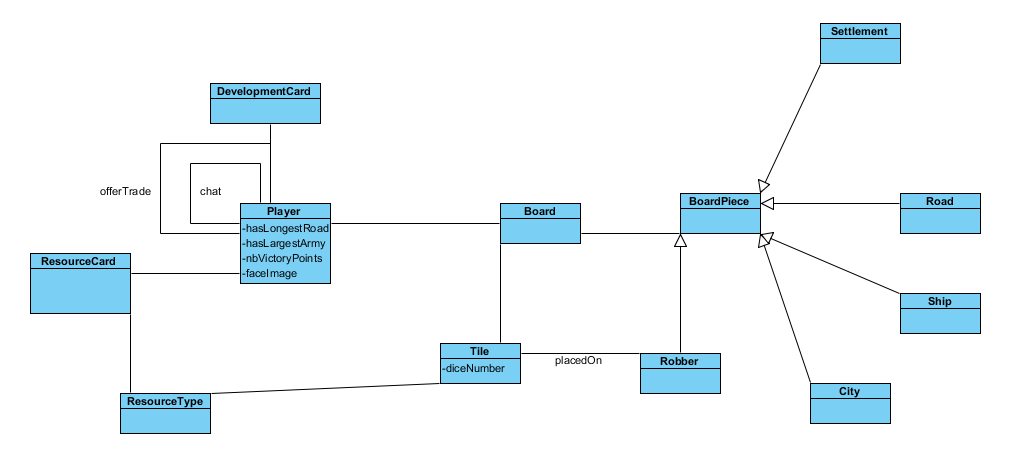
\includegraphics[width=1\textwidth]{Image/Ontwerp/DomainModel.png}
\caption{Domain model}
\label{fig:empty}
\end{center}
\end{figure}

\subsection{SOC.client package}
This package contains the code that makes up the Graphical User Interface.

The SOC.client package revolves around 3 God classes: SOCPlayerInterface, SOCHandPanel and SOCPlayerClient. 
They all contain dependencies to eachother. 
The remainder of the classes of this package can be divided into 2 parts. 
One part consists of helper classes used for user interface rendering. 
The other part contains mainly dialogs that are presented to the user and some panels that display a part of the game state. 
Almost all classes depend on one or more of the 3 god classes. 
In turn the 3 godclasses use all these parts to build the Client Interface.

\begin{figure}
\begin{center}
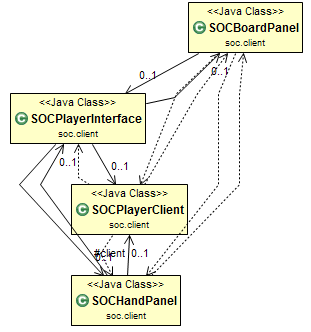
\includegraphics[width=0.4\textwidth]{Image/Ontwerp/ClientCore.png}
\caption{SOC.Client package overview}
\label{fig:empty}
\end{center}
\end{figure}

\subsection{SOC.game package}
This package holds the game state and data. 
A large part of this package contains a very complicated but seemingly ingenious way to work with the game board. 
(This is due to the board being hexagonal and board pieces being placed at corners or edges of tiles)

The main class in this package is the SOCGame class. 
It literally uses ALL other classes in this package. 
The class is used to store current game state and the game board, among other features.

\newpage

\section{Evaluatie ontwerp}

Maaanyy godclasses

The design structures that are present in the project seem to have been added while coding. 
There are some inheritance hierarchies present but it is not used for polymorfysm 

\section{Patronen}

\newpage

\section{Analysetools}

\subsection{Coverlipse}

\newpage

\section{Testen}

\newpage

\section{Besluit}

Hello 


\newpage

\section{Projectbeheer}

\end{document}